\chapter{Platform Driver Labor Supply Beyond Earnings Maximization}\label{chap:jakarta}
\epigraph{Most of the elasticities we estimate are nega- tive; drivers tend to quit early on high wage days and to drive longer hours on low wage days.}{\cite{Camerer1997}}
 This chapter analyzes data from a survey in Jakarta and shows that drivers do not purely maximize their earnings in their labor supply choices. In an analysis of free-text answers, we highlight understanding of the app and information as important determinants of driver behavior.
\section{Survey}
Our data comes from a survey conducted in spring 2021 in Jakarta, Indonesia.
\subsection{Sample}
Participants were asked to complete an online survey hosted on Qualtrics. 846 complete survey responses were submitted. We excluded from the analysis drivers that stated more than 16 hours of work per day and stated earnings smaller than 10,000 Rp or larger than 2,000,000 Rp. The survey participants were recruited through social media via two platform driver \emph{WhatsApp} groups.

\autoref{fig:age} shows the age distribution of participants. Note that about 50\% of drivers are within the age group of 30 to 39. About 97.5\% of drivers who participated in the survey identify as male, 2.5\% identify as female. Around 97\% are motorbike delivery drivers, the other 3\% drive cars.

Three major ride-hailing companies operate in Jakarta: Grab, GoJek and Shopee. While Grab and GoJek are incumbents in this market, Shoppee entered the market only in 2021. Around 94\% of drivers work for the incumbents Grab or GoJek. In our sample of drivers, only 12\% of the respondents in the survey are multi-homers. 
\begin{table}[!ht]
\centering
 \begin{tabular}{cccccc}	
 \toprule
 Age Group&<20&20-29&30-39&40-49&>50\\
 \midrule
 Proportion&2\%&27\%&49\%&20\%&3\%\\
 \bottomrule	
 \end{tabular}
 \caption{Age Distribution of respondents}\label{tab:agedistr}
 \end{table}
\subsection{Questions}
 The survey consists of multiple questions blocks and is reproduced in its entirety in Appendix~\ref{appendix:survey}. 

In a first block, participants were asked to check all TNCs they have worked for in the past 30 days. A survey respondent is defined as a \emph{multi-homer} if they have been working for at least two platforms in the past 30 days. In this first block, basic information and driving behavior are asked as well, e.g., vehicle type used, previous occupation, behaviors while waiting for the next order.

The second block's questions differ for multi-homers and non-multi-homers. Multi-homers are asked how they switch between different platforms, allocations of their working hours and reasons for multi-homing. For non-multi-homers, reasons for non-multi-homing and factors that would make them multi-home are elicited.

In a third block, for each ride-hailing platform survey participants have worked for in the last 30 days, respondents are asked questions about their labor supply choices. Type of work (delivery, ridesourcing), part of the city of highest activity, and daily working hours, distance, and earnings.

A final block elicited socio-demographic information, including age, gender, educational status, income level, living areas, and weekly expenses. 
\section{Descriptive Evidence}
A first observation we make is that there is significant correlation between experience working as a taxi driver before and multi-homing behaviors. The OLS regression model shown in Table \ref{tab:opang} suggests that drivers who has been motorcycle taxi drivers before are less likely to multi-home in Jakarta market.
 \begin{table}
 \centering
     \caption{Results of regression models predicting multi-homing behaviors of ride-hailing drivers in Jakarta based on previous occupation}
         \begin{tabular}{lcccccc}
         \toprule
         \textbf{Variable} & \textbf{coef} & \textbf{std err} & \textbf{t} & \textbf{P$> |$t$|$} & \textbf{[0.025} & \textbf{0.975]}  \\
         \midrule
         \textbf{Intercept} &       0.1276***  &        0.012     &    10.735  &         0.000        &        0.104    &        0.151     \\
         \textbf{Former taxi driver}     &      -0.0796**  &        0.031     &    -2.574  &         0.010        &       -0.140    &       -0.019     \\
         \midrule
         \multicolumn{1}{r}{\textbf{R-squared: }}   & 0.008 & \multicolumn{3}{c}{\textbf{Adjusted R-squared: }}  & 0.007 & \\
         \bottomrule 
         \end{tabular}
     \label{tab:opang}
 \end{table}

 There is also a weak effect of (self-reported) part-time status and multi-homing, \autoref{tab:part-timer}. Part-time ride-hailing drivers are more likely to multi-home than full-time drivers. 

 \begin{table}
 \centering
     \caption{Results of regression models predicting multi-homing behaviors of ride-hailing drivers in Jakarta based on whether being part-time ride-hailing drivers}
         \begin{tabular}{lcccccc}
         \toprule
         \textbf{Variable} & \textbf{coef} & \textbf{std err} & \textbf{t} & \textbf{P$> |$t$|$} & \textbf{[0.025} & \textbf{0.975]}  \\
         \midrule
         \textbf{Intercept}                           &       0.1097***  &        0.012     &     9.258  &         0.000        &        0.086    &        0.133     \\
         \textbf{Part-Time} &       0.0441  &        0.032     &     1.384  &         0.167        &       -0.018    &        0.107     \\
         \midrule
         \multicolumn{1}{r}{\textbf{R-squared: }}   & 0.002 & \multicolumn{3}{c}{\textbf{Adjusted R-squared: }}  & 0.001 & \\
         \bottomrule 
         \end{tabular}
     \label{tab:part-timer}
 \end{table}
 \section{Earnings for Different Platforms}
Our main finding concerns the earnings for different platforms. Figure \ref{fig:hourly_salary} displays the hourly salary distribution of all survey respondents in Jakarta. The median respondent makes less than 20,000 Rp (approximately \$ 1.40) per hour, which is significantly less than the average hourly salary 120,175 Rp (approximately \$ 8.4) in Jakarta~\cite{Jakarta_hourly_salary}.

 \begin{figure}
     \centering
     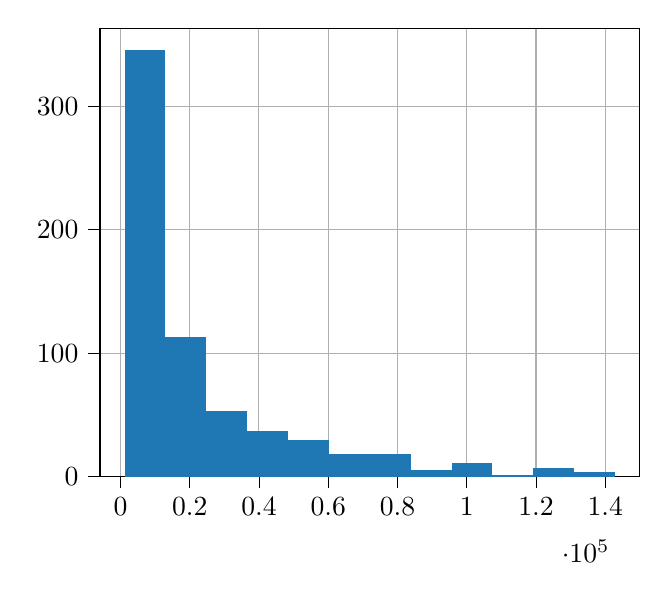
\begin{tikzpicture}

\definecolor{color0}{rgb}{0.12156862745098,0.466666666666667,0.705882352941177}

\begin{axis}[
tick align=outside,
tick pos=left,
x grid style={white!69.0196078431373!black},
xmajorgrids,
xmin=-5900.35714285714, xmax=149940.833333333,
xtick style={color=black},
y grid style={white!69.0196078431373!black},
ymajorgrids,
ymin=0, ymax=363.3,
ytick style={color=black}
]
\draw[draw=none,fill=color0,line width=0.32pt] (axis cs:1183.33333333333,0) rectangle (axis cs:12989.4841269841,346);
\draw[draw=none,fill=color0,line width=0.32pt] (axis cs:12989.4841269841,0) rectangle (axis cs:24795.6349206349,113);
\draw[draw=none,fill=color0,line width=0.32pt] (axis cs:24795.6349206349,0) rectangle (axis cs:36601.7857142857,53);
\draw[draw=none,fill=color0,line width=0.32pt] (axis cs:36601.7857142857,0) rectangle (axis cs:48407.9365079365,37);
\draw[draw=none,fill=color0,line width=0.32pt] (axis cs:48407.9365079365,0) rectangle (axis cs:60214.0873015873,30);
\draw[draw=none,fill=color0,line width=0.32pt] (axis cs:60214.0873015873,0) rectangle (axis cs:72020.2380952381,18);
\draw[draw=none,fill=color0,line width=0.32pt] (axis cs:72020.2380952381,0) rectangle (axis cs:83826.3888888889,18);
\draw[draw=none,fill=color0,line width=0.32pt] (axis cs:83826.3888888889,0) rectangle (axis cs:95632.5396825397,5);
\draw[draw=none,fill=color0,line width=0.32pt] (axis cs:95632.5396825397,0) rectangle (axis cs:107438.69047619,11);
\draw[draw=none,fill=color0,line width=0.32pt] (axis cs:107438.69047619,0) rectangle (axis cs:119244.841269841,1);
\draw[draw=none,fill=color0,line width=0.32pt] (axis cs:119244.841269841,0) rectangle (axis cs:131050.992063492,7);
\draw[draw=none,fill=color0,line width=0.32pt] (axis cs:131050.992063492,0) rectangle (axis cs:142857.142857143,4);
\end{axis}

\end{tikzpicture}
     \caption{Hourly salary distribution of survey respondents}
     \label{fig:hourly_salary}
 \end{figure}

We estimate, among all single-homers, the correlation between working for GoJek and hourly salary in Table \ref{tab:hourly_salary}. We exclude the 3\% of non-motorcycle drivers due to their significantly different earnings. The model results suggest that GoJek drivers earn significantly less than drivers from other platforms, 11,000 Rp (approximately \$ 0.77) less per hour. While a weak effect ($R^2 = 0.002$), the difference is highly significant. This result stands also when controlling for age, gender, school diploma, and previous experience as a taxi driver.

\begin{table}[!htbp] \centering
\begin{tabular}{@{\extracolsep{5pt}}lcc}
\\[-1.8ex]\hline
\hline \\[-1.8ex]
& \multicolumn{2}{c}{\textit{Dependent variable:}} \
\cr \cline{2-3}
\\[-1.8ex] & without controls & with controls \\
\hline \\[-1.8ex]
 Intercept & 30713.817$^{***}$ & 32141.158$^{***}$ \\
  & (1927.295) & (10919.276) \\
% Q54[T.30 - 39] & & 599.344$^{}$ \\
%  & & (9829.024) \\
% Q54[T.30 - 39]:Q58[T.Yes] & & -1459.150$^{}$ \\
%  & & (10215.505) \\
% Q54[T.40 - 49] & & -5300.705$^{}$ \\
%  & & (13705.572) \\
% Q54[T.40 - 49]:Q58[T.Yes] & & 2649.267$^{}$ \\
%  & & (14135.068) \\
% Q54[T.Above 50] & & -655.081$^{}$ \\
%  & & (17545.153) \\
% Q54[T.Above 50]:Q58[T.Yes] & & 3628.347$^{}$ \\
%  & & (19003.614) \\
% Q54[T.Under 20] & & -689.077$^{}$ \\
%  & & (4819.356) \\
% Q54[T.Under 20]:Q58[T.Yes] & & -689.077$^{}$ \\
%  & & (4819.356) \\
% Q55[T.Male] & & -5813.134$^{}$ \\
%  & & (4617.561) \\
% Q55[T.Prefer not to answer] & & -17966.204$^{}$ \\
%  & & (19349.857) \\
% Q57[T.None of the above] & & -0.000$^{}$ \\
%  & & (0.000) \\
% Q57[T.S1 or higher] & & -5956.143$^{}$ \\
%  & & (7460.034) \\
% Q57[T.SD] & & 6745.220$^{}$ \\
%  & & (8008.309) \\
% Q57[T.SMA] & & -338.772$^{}$ \\
%  & & (5669.506) \\
% Q57[T.SMP] & & 1058.908$^{}$ \\
%  & & (6598.707) \\
% Q58[T.Yes] & & 5170.436$^{}$ \\
%  & & (8691.783) \\
 gojek[T.True] & -11001.520$^{***}$ & -10506.619$^{***}$ \\
  & (2366.886) & (2426.682) \\
\hline \\[-1.8ex]
 Observations & 552 & 552 \\
 $R^2$ & 0.038 & 0.052 \\
 Adjusted $R^2$ & 0.036 & 0.025 \\
% Residual Std. Error & 26284.803(df = 550) & 26435.066(df = 536)  \\
% F Statistic & 21.605$^{***}$ (df = 1.0; 550.0) & 1.942$^{**}$ (df = 15.0; 536.0) \\
\hline
\hline \\[-1.8ex]
\textit{Note:} & \multicolumn{2}{r}{$^{*}$p$<$0.1; $^{**}$p$<$0.05; $^{***}$p$<$0.01} \\
\end{tabular}
\caption{Results of regression models predicting hourly earnings of platform drivers drivers in Jakarta based on whether working for GoJek}\label{tab:working_hours}
\end{table}


For the same group of drivers, we consider the difference of total working hours between ride-hailing platforms.
 The model results in Table \ref{tab:working_hours} show that GoJek drivers work significantly longer than drivers from other platforms, 0.866 hours more per day, when controlling for age, gender, school diploma, and previous experience as a taxi driver. 
 
 Both regression results imply that drivers must optimize for other factors besides earnings. We investigate free-text answers to close this chapter.
 
 \begin{table}[!htbp] \centering
\begin{tabular}{@{\extracolsep{5pt}}lcc}
\\[-1.8ex]\hline
\hline \\[-1.8ex]
& \multicolumn{2}{c}{\textit{Dependent variable:}} \
\cr \cline{2-3}
\\[-1.8ex] & without controls & with controls \\
\hline \\[-1.8ex]
 Intercept & 10.664$^{***}$ & 8.328$^{***}$ \\
  & (0.162) & (0.874) \\
% Q54[T.30 - 39] & & -0.761$^{}$ \\
%  & & (0.791) \\
% Q54[T.30 - 39]:Q58[T.Yes] & & 0.970$^{}$ \\
%  & & (0.829) \\
% Q54[T.40 - 49] & & -1.880$^{*}$ \\
%  & & (1.072) \\
% Q54[T.40 - 49]:Q58[T.Yes] & & 1.916$^{*}$ \\
%  & & (1.116) \\
% Q54[T.Above 50] & & -1.056$^{}$ \\
%  & & (1.440) \\
% Q54[T.Above 50]:Q58[T.Yes] & & 1.595$^{}$ \\
%  & & (1.572) \\
% Q54[T.Under 20] & & 1.204$^{}$ \\
%  & & (2.642) \\
% Q54[T.Under 20]:Q58[T.Yes] & & -2.903$^{}$ \\
%  & & (2.785) \\
% Q55[T.Male] & & 0.928$^{**}$ \\
%  & & (0.395) \\
% Q55[T.Prefer not to answer] & & 1.378$^{}$ \\
%  & & (1.523) \\
% Q57[T.None of the above] & & -0.000$^{}$ \\
%  & & (0.000) \\
% Q57[T.S1 or higher] & & -0.198$^{}$ \\
%  & & (0.603) \\
% Q57[T.SD] & & 0.073$^{}$ \\
%  & & (0.698) \\
% Q57[T.SMA] & & -0.032$^{}$ \\
%  & & (0.480) \\
% Q57[T.SMP] & & 0.063$^{}$ \\
%  & & (0.568) \\
% Q58[T.Yes] & & 1.749$^{**}$ \\
%  & & (0.689) \\
 gojek[T.True] & 1.033$^{***}$ & 0.866$^{***}$ \\
  & (0.210) & (0.206) \\
\hline \\[-1.8ex]
 Observations & 655 & 655 \\
 $R^2$ & 0.036 & 0.136 \\
 Adjusted $R^2$ & 0.034 & 0.114 \\
% Residual Std. Error & 2.648(df = 653) & 2.536(df = 638)  \\
% F Statistic & 24.120$^{***}$ (df = 1.0; 653.0) & 6.273$^{***}$ (df = 16.0; 638.0) \\
\hline
\hline \\[-1.8ex]
\textit{Note:} & \multicolumn{2}{r}{$^{*}$p$<$0.1; $^{**}$p$<$0.05; $^{***}$p$<$0.01} \\
\end{tabular}
\caption{Results of regression models predicting daily working hours of ride-hailing drivers in Jakarta based on whether working for GoJek}\label{tab:hourly_salary}
\end{table}

\section{Free-Text}
 In this section, we use a fine-tuned language model \cite{Devlin2019} to predict whether single-homing drivers drive for two of the bigger companies Grab and GoJek. We then use the global feature importance metric SHAP \cite{Lundberg2017} to determine topics that might motivate drivers working for a platform that guarantees them more earning vs. the other. 
 
 All of the analysis is use answers to question 16 (compare Appendix~\ref{appendix:survey}) \enquote{Anything else we should know about why you decided not to use multiple platforms?}.

We fine-tuned a natural language model BERT \cite{Devlin2019} trained on the Indonesian Wikipedia. The output of our model can be found in \autoref{app:kdd}

The words most indicative of working for GoJek, the platform with lower reported earnigns, are

\begin{table}
\centering
\begin{tabular}{ccc}
\toprule
&&\\
\midrule
&&\\
\bottomrule	
\end{tabular}
\caption{Sum of Feature Importance in SHAP scores}	
\end{table}

%gridwise: Using across platforms
%vehicle requirements
%bounced out
%focus/confusion
%indonesian incumbent
\section{Discussion}
We find significant earnings and working hours differences between single-homing drivers. The majority of respondents works for a platform where they report longer working hours and less hourly wages.

In our analysis of free-text answers, we find that drivers working for a lower-paying platform cite informational and cultural reasons for their choice. 

The prevalence of information as a reason of drivers for the less-earning platform leads to the next chapter, which gives additional  The value of demand information, whose design we are going to study in \autoref{chap:infodesign} is part of our analysis the next chapter.
